\documentclass[11pt]{article}

% Usepackages 

\usepackage[utf8]{inputenc}
\usepackage[hmargin={1.5 cm,1.5cm},
   top=1.5cm, marginpar=3.5cm, bottom=1.5cm
   ]{geometry}  
\usepackage{subfiles}
\usepackage{hyperref}
\usepackage{physics}
\usepackage[most]{tcolorbox}
\usepackage{xparse}
\usepackage{accents}
\usepackage{pdfpages}
\usepackage{wrapfig}
\usepackage{amsmath}
\usepackage{amssymb}
\usepackage{amsthm}
\usepackage{amsfonts}
\usepackage{mathrsfs}
\usepackage{listings}
\usepackage{xcolor}
\usepackage{bbm}
\usepackage{tikz-cd}
\usepackage{tikz}
\usepackage{mathtools}
\usepackage{pgfplots}
\usepackage{titlesec}
\usetikzlibrary{arrows}
\pgfplotsset{width=7cm,height=9cm,plotstyle/.style={line width=1.2pt,smooth,samples=100,domain=-0.05:1.01}} 

%%%%%%%%

%Bibliography

%\addbibresource{ref.bib}

%%%%%%%%%

% Additional Styles

\hypersetup{colorlinks = true, linkcolor = blue, urlcolor = violet}

%\titleformat{\chapter}[display]{\normalfont\sffamily\Large\bfseries\centering}{\chaptertitlename\ \thechapter}{0pt}{\Huge}

\titleformat{\section}[hang]{\fontsize{14}{15}\sffamily\bfseries\centering}{\color{columbiablue}\S}{0.21em}{}

\newcommand{\textscf}[1]{\textbf{\textsc{#1}}}
%%%%%%
\definecolor{deepjunglegreen}{rgb}{0.40, 0.69, 0.29}
\definecolor{columbiablue}{rgb}{0.41, 0.37, .84}
%Theorem Box

\newtcbtheorem[no counter]{Thm}{\textbf{Theorem}}{
  breakable, enhanced,
  attach boxed title to top left={xshift=3mm, yshift=-3mm, yshifttext=-1mm},
  fonttitle=\sffamily,
  coltitle=blue!70,
  colbacktitle=white,
  %colbacktitle=cosmiclatte,
  colback=cyan!6,
  colframe=black!70,
  leftrule=0.5mm,
  rightrule=0.2mm,
  toprule=0.2mm,
  bottomrule=0.2mm,
  separator sign none, description delimiters parenthesis,
  description font=\mdseries}{th}

% defination Box

\newtcbtheorem[number within=section]{Def}{Definition}{
  breakable, enhanced,
  attach boxed title to top left={xshift=3mm, yshift=-3mm, yshifttext=-1mm},
  coltitle=black,
  colbacktitle=columbiablue!25,
  fonttitle=\sffamily,
  colback=white,
  colframe=black,
  leftrule=0.5mm,
  rightrule=0.2mm,
  toprule=0.2mm,
  bottomrule=0.2mm,
  arc=2.5mm,
  separator sign={\ $\blacktriangleright$},
  description delimiters none,
  description font=\bfseries}{def}

%Lemma
\definecolor{electricviolet}{rgb}{0.56, 0.0, 1.0}

\newtcbtheorem[no counter]{Lem}{ \textbf{\textcolor{electricviolet}{\S} Lemma:}}{
  detach title,
  fonttitle=\sffamily,
  coltitle=black,
  colbacktitle=white,
  colback=white,
  colframe=white,
  description font=\bfseries,
  before upper={\tcbtitle},
  title = $\mathbf{\S}$ \textsc{Lemma}
}{}

\newtcbtheorem[number within=section]{Lemn}{ \textbf{\textcolor{deepjunglegreen}{\S} Lemma}}{
  detach title,
  fonttitle=\sffamily,
  coltitle=black,
  colbacktitle=white,
  colback=white,
  colframe=white,
  description font=\bfseries,
  before upper={\tcbtitle},
  title = $\mathbf{\S}$ \textsc{Lemma}
}{}

%%% Info box 
\definecolor{corn}{rgb}{0.98, 0.93, 0.36}
\definecolor{awesome}{rgb}{1.0, 0.13, 0.32}
\definecolor{verdigris}{rgb}{0.26, 0.7, 0.68}
\definecolor{ufogreen}{rgb}{0.24, 0.82, 0.44}
\definecolor{turquoiseblue}{rgb}{0.0, 1.0, 0.94}
\definecolor{salmonpink}{rgb}{1.0, 0.57, 0.64}
\definecolor{screamin}{rgb}{0.46, 1.0, 0.44}
\newtcbtheorem[no counter]{Sly}{}{
 breakable, enhanced,
%   attach boxed title to top left={xshift=3mm, yshift= -3mm, yshifttext=-1mm},
  %coltitle=black,
  %colbacktitle=cyan!70,
  fonttitle=\sffamily,
  colback=cyan!5,
  colframe=black,
  leftrule=0.2mm,
  rightrule=0.2mm,
  toprule=0.2mm,
  bottomrule=0.2mm,
  separator sign none,
  description font=\bfseries}{}

%%%%%


%%%%problems
\definecolor{bondiblue}{rgb}{0.0, 0.58, 0.71}

\newtcbtheorem[no counter]{prob}{\textcolor{bondiblue}{\textbf{\textsf{Problem.}}}}{
  detach title,
  fonttitle=\sffamily,
  coltitle=black,
  colbacktitle=white,
  colback=white,
  colframe=white,
  leftrule=0.1mm,
  rightrule= -0.1mm,
  toprule=-0.1mm,
  bottomrule=-0.1mm,
  description font=\bfseries,
  before upper={\tcbtitle},
  title = $\mathbf{\S}$ 
}{}




% Main documentclass

\newcommand{\bb}[1]{\mathbb{#1}}
\newcommand{\N}{\bb{N}}
\newcommand{\Z}{\bb{Z}}
\newcommand{\Q}{\bb{Q}}
\newcommand{\R}{\mathbb{R}}
\newcommand{\C}{\bb{C}}
\newcommand{\Op}[1]{\mathcal{O}_{#1}}
\newcommand{\msk}{\medskip}
\newcommand{\ssk}{\smallskip}
\newcommand{\bsk}{\bigskip}
\newcommand{\Qed}{\quad \blacksquare}
\newcommand{\contra}{\rightarrow \leftarrow}
\newcommand{\heart}{\ensuremath\heartsuit}
\newcommand{\butt}{\rotatebox[origin=c]{180}{\heart}}
\newcommand{\ltag}[2]{\label{#1} \tag{#2}}
\newcommand{\floor}[1]{\lfloor {#1} \rfloor}
\newcommand{\inp}[2]{\left\langle {#1}, {#2} \right\rangle}
\newcommand{\vphi}{\varphi}
\newcommand{\veps}{\varepsilon}
\newcommand{\pdot}[2]{{#1} \cdot {#2}}
\newcommand{\Area}{\operatorname{Area}}
\newcommand{\ran}{\operatorname{ran}}
\newcommand{\Vol}{\operatorname{Vol}} 
\newcommand{\s}{\bb{S}}
\newcommand{\fb}[1]{\mathbf{#1}}
\newcommand{\T}{\mathbf{Top}}
\newcommand{\p}{\partial}
\newcommand{\ch}{\mathbf{Chain}^*}
\newcommand{\cha}{\mathbf{Chain}^\text{ag}}
\newcommand{\gr}{\mathbf{Graded groups}}
\newcommand{\kc}{\mathcal{K}}
\newcommand{\D}{\Delta}
\newcommand{\de}{\delta}
\newcommand{\ep}{\varepsilon}
\newcommand{\coro}[1]{{\hspace*{0.6cm} \textcolor{purple}{\textsc{Corollary. }}}\textit{#1}}
\newcommand{\examp}{\hspace{0.6cm} $\blacklozenge$ \textsc{Example} \textbf{:}} 
\newcommand{\ts}[1]{\textbf{\textsf{#1}}}
\newcommand{\cod}[1]{\textcolor{codegreen}{\texttt{#1}}}
\newcommand{\F}{\mathbb{F}}
\newcommand{\theo}[2]{{\hspace*{0.6cm} \textcolor{blue}{\textsc{Theorem.}}\hspace*{0.1cm}\textbf{\textsf{#1}} \hspace*{0.1cm}}\textit{#2}}
\newcommand{\sol}{ \textbf{\textit{Solution.}} }
\newcommand{\id}{\mathrm{id}}
%%%%%% 

\definecolor{codegreen}{rgb}{0,0.6,0}
\definecolor{codegray}{rgb}{0.5,0.5,0.5}
\definecolor{codepurple}{rgb}{0.58,0,0.82}
\definecolor{backcolour}{rgb}{1,1,1}

\lstdefinestyle{mystyle}{
    backgroundcolor=\color{backcolour},   
    commentstyle=\color{blue},
    keywordstyle=\color{magenta},
    numberstyle=\tiny\color{codegray},
    stringstyle=\color{codepurple},
    basicstyle=\ttfamily\footnotesize,
    breakatwhitespace=false,         
    breaklines=true,                 
    captionpos=b,                    
    keepspaces=true,                 
    numbers=left,                    
    numbersep=5pt,                  
    showspaces=false,                
    showstringspaces=false,
    showtabs=false,                  
    tabsize=2
}

\lstset{style=mystyle}


%%%%%%%

\begin{document}
 
 \title{{\Huge \textsc{Assignment-3}}}
 \author{\textbf{ \textsf{Algebraic Topology}} \\[0.2cm]
 \large \textsc{Trishan Mondal}}
 \date{}
 \maketitle

 ----------------------------------------------------------------------------------------------------------------------------------------- 

 \section{Problem 1} 

 \begin{prob}{}{}
    Consider a commutative diagram of abelian groups:

    \[\begin{tikzcd}
        \cdots & {A_n} & {B_n} & {C_n} & {A_{n-1}} & \cdots \\
        \cdots & {A_n'} & {B_n'} & {C_n'} & {A_{n-1}'} & \cdots
        \arrow[from=1-5, to=1-6]
        \arrow[from=2-5, to=2-6]
        \arrow[from=1-1, to=1-2]
        \arrow[from=2-1, to=2-2]
        \arrow["{f_n}", from=1-2, to=1-3]
        \arrow["{g_n}", from=1-3, to=1-4]
        \arrow["{\p_n}", from=1-4, to=1-5]
        \arrow["{f'_n}", from=2-2, to=2-3]
        \arrow["{g'_n}", from=2-3, to=2-4]
        \arrow["{\p'_n}", from=2-4, to=2-5]
        \arrow["{a_n}"', from=1-2, to=2-2]
        \arrow["{b_n }", from=1-3, to=2-3]
        \arrow["{c_n}", color={rgb,255:red,36;green,76;blue,255}, from=1-4, to=2-4]
        \arrow["{a_{n-1}}", from=1-5, to=2-5]
    \end{tikzcd}\]
    where the rows are long exact sequences and $c_{n}$ is an isomorphism for all $n \in \mathbb{Z}$. Verify that the associated ``algebraic Mayer-Vietoris" sequence:
   \[\begin{tikzcd}
	\cdots & {A_n} & {A_n'\oplus B_n} & {B_n'} & {A_{n-1}} & \cdots
	\arrow[from=1-5, to=1-6]
	\arrow[from=1-1, to=1-2]
	\arrow["{(a_n,-f_n)}", from=1-2, to=1-3]
	\arrow["{(f_n'+b_n)}", from=1-3, to=1-4]
	\arrow["{\p^{MV}_n}", from=1-4, to=1-5]
     \end{tikzcd}
    \] 
    is exact, where $\partial_{n}^{M V}:=\partial_{n} \circ c_{n}^{-1} \circ g_{n}^{\prime}$.
 \end{prob} 

 \sol Let $\psi_n = (a_n, -f_n)$ and let $\phi_n = \begin{pmatrix} f_n' \\ b_n \end{pmatrix}$. To show that the \textsf{algebraic Mayer-Vietoris sequence} is exact its enough to show that $\operatorname{Im}\psi_n = \ker\phi_n$, $\operatorname{Im} \phi_n = \ker\p^{MV}_n$ and $\operatorname{Im}\p_n^{MV} = \ker\psi_{n-1}$.

 \begin{itemize}
     \item $\mathbf{\operatorname{Im}\psi_n = \ker\phi_n}$. Let $x \in A_n$, we have
     \begin{align*}
         \phi_n(\psi_n(x)) = f'_n(a_n(x)) - b_n(f_n(x)) = 0.
     \end{align*}
     Thus $\operatorname{Im}\psi_n \subseteq \ker\phi_n$. For opposite inclusion suppose $(x',y) \in \ker\phi_n$, then we get that $f'_n(x') = -b_n(y)$, but then we get 
     \[
         0 = g'_n(f'_n(x') + b_n(y)) = g'_n(b_n(y)) = c_n(g_n(y)) \Rightarrow g_n(y) = 0,    
     \]
     since $c_n$ is an isomorphism. Thus we get that $y \in \ker g_n = \operatorname{Im} f_n$, let $y = f_n(a)$. Then we get that 
     \begin{align*}
         f'_n(a_n(a)+x') &= f'_n(a_n(a)) + f'_n(x') \\ &= b_n(f_n(a)) + f'_n(x') \\ &= b_n(y)+f'_n(x') = 0.
     \end{align*}
     Hence $a_n(a) + x' \in \ker f'_n = \operatorname{Im} \p'_{n+1}$, let $a_n(a)+x' = \p'_{n+1}(z')$. Now since $c_{n+1}$ is an isomorphism we get there exists $z \in C_{n+1}$ such that 
     \begin{align*}
         a_n(a) + x' = \p'_{n+1}(z') = \p'_{n+1}(c_{n+1}(z)) = a_n(\p_{n+1}(z)).
     \end{align*}
     Let $\widetilde{a} = \p_{n+1}(z) - a$, then we get that $a_n(\widetilde{a}) = x'$ and $f_n(\widetilde{a}) = f_n(\p_{n+1}(z)) - f_n(a) = -y$. Hence we get that $\psi_n(\widetilde{a}) = (x',y)$. Therefore we have shown that $\operatorname{Im} \psi_n = \ker \phi_n$.
 
     \item $\mathbf{\operatorname{Im} \phi_n = \ker\p^{MV}_n}$. Let $(x',y) \in A'_n \oplus B_n$, then we get that 
     \begin{align*}
         \p_n^{MV}(\phi_n(x',y)) &= \p_n^{MV}(f'_n(x')) + \p^{MV}_n(b_n(y)) \\ 
         &= \p_n(c_n^{-1}g'_n(f'_n(x'))) + \p_n(c_n^{-1}g'_n(b_n(y))) \\ 
         &= \p_n(c_n^{-1}(0)) + \p_n(g_n(y)) = 0.
     \end{align*}
     Thus we get that $\operatorname{Im}\phi_n \subseteq \ker\p_n^{MV}$. Conversely suppose $y' \in \ker\p^{MV}_n$, then we get 
     \begin{align*}
         \p_n(c^{-1}_n(g'_n(y'))) = 0 \Rightarrow c_n^{-1}(g_n'(y')) \in \ker\p_n = \operatorname{Im} g_n.
     \end{align*}
     Thus there exists $y \in B_n$ such that 
     \begin{align*}
         c_n^{-1}(g_n'(y')) = g_n(y) \Rightarrow g_n'(y') = c_n(g_n(y)) = g_n'(b_n(y)).
     \end{align*}
     Hence $y' - b_n(y) \in \ker g_n' = \operatorname{Im} f_n'$, thus there exists $x' \in A_n'$ such that 
     \begin{align*}
         y' - b_n(y) = f_n'(x') \Rightarrow y' = f'_n(x') + b_n(y).
     \end{align*}
     Hence we get that $\ker\p^{MV}_n \subseteq \operatorname{Im}\phi_n$, therefore we have shown that $\operatorname{Im}\phi_n = \ker\p^{MV}_n$. 
 
     \item $\mathbf{\operatorname{Im} \p_n^{MV} = \ker\psi_{n-1}}$. Let $y' \in B_n'$, then we get that 
     \begin{align*}
         \psi_{n-1}(\p_n^{MV}(y')) &= (a_{n-1}(\p_n(c_n^{-1}(g_n'(y')))), -f_{n-1}(\p_n(c_n^{-1}(g_n'(y'))))) \\ 
         &= (\p_n'(g_n'(y')),0) = (0,0).
     \end{align*}
     Thus $\operatorname{Im}\p^{MV}_n \subseteq \ker\psi_{n-1}$. Conversely let $x \in \ker\psi_{n-1}$, then we get that $a_{n-1}(x) = 0$ and $f_{n-1}(x) = 0$. But then we get $x \in \ker f_{n-1} = \operatorname{Im} \p_n$, thus $x = \p_n(z)$ for some $z \in C_n$. Now observe that 
     \begin{align*}
         0 = a_{n-1}(x) = a_{n-1}(\p_n(z)) = \p_n'(c_n(z)) = 0 \Rightarrow c_n(z) \in \ker\p_n' = \operatorname{Im} g_n'. 
     \end{align*} 
     But then we get $c_n(z) = g_n'(y') \Rightarrow z = c_n^{-1}(g_n'(y'))$ and hence we get $x = \p_n(c_n^{-1}(g_n'(y'))) \in \operatorname{Im} \p^{MV}_n$. Therefore have shown that $\ker\psi_{n-1} \subseteq \operatorname{Im} \p_n^{MV} \Rightarrow \operatorname{Im} \p^{MV}_n = \ker\psi_{n-1}$.
 \end{itemize}
 Therefore we have proved that the \textsf{algebraic Mayer-Vietoris sequence} is exact. $\hfill \blacksquare$


 \section{Problem 2}

 \begin{prob}{}{}
    Compute the homology groups of the surfaces $\Sigma_{g}$ for all $g \geq 0$. Compute their Betti numbers.
 \end{prob}

 \sol We have proved the polygonal presentation $\Sigma_g$ in \textbf{Assignment 2}. Consider the $4g$-gon (call it $P$) whose edges are identified with the following identification as shown in figure. Let, $D$ be a  point at the center of the $4g$-gon. Take the open set $P \setminus D$,  let $V$ be the open set corresponding open set in $\Sigma_g$ and $U$ be the open set containing $D$ in $P$, it will remain same in the quotient space $\Sigma_g$. We can see $U \subseteq \bar{V}$, thus we can use Mayer-Vietoris sequence on the open cover $U \cup V$. It's not hard to see $\Sigma_g = U \cup V$, $U \cap V = U \setminus D$,which deformation retracts on to a circle $\s^1$.   

\begin{figure}[htbp]
   \centering
   

\tikzset{every picture/.style={line width=0.75pt}} %set default line width to 0.75pt        

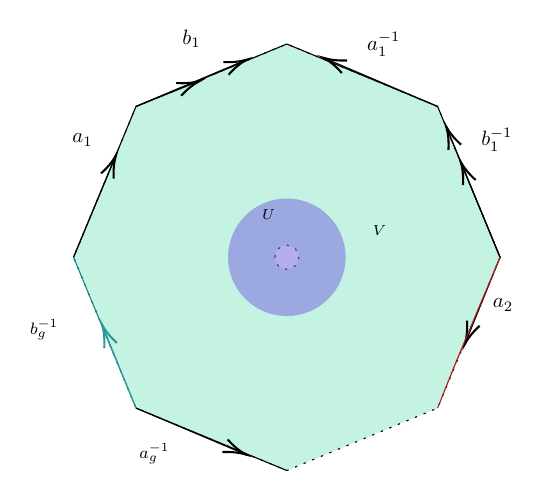
\begin{tikzpicture}[x=0.75pt,y=0.75pt,yscale=-1,xscale=1]
%uncomment if require: \path (0,268); %set diagram left start at 0, and has height of 268

%Shape: Regular Polygon [id:dp41014614704630903] 
\draw  [fill={rgb, 255:red, 188; green, 241; blue, 222 }  ,fill opacity=0.88 ][dash pattern={on 0.84pt off 2.51pt}] (452,129.75) -- (421.91,202.41) -- (349.25,232.5) -- (276.59,202.41) -- (246.5,129.75) -- (276.59,57.09) -- (349.25,27) -- (421.91,57.09) -- cycle ;
%Straight Lines [id:da5179448077631912] 
\draw    (246.5,129.75) -- (258.52,100.88) -- (266.23,82.35) ;
\draw [shift={(267,80.5)}, rotate = 112.6] [color={rgb, 255:red, 0; green, 0; blue, 0 }  ][line width=0.75]    (10.93,-3.29) .. controls (6.95,-1.4) and (3.31,-0.3) .. (0,0) .. controls (3.31,0.3) and (6.95,1.4) .. (10.93,3.29)   ;
%Straight Lines [id:da14683792457808598] 
\draw    (276.59,57.09) -- (328.16,35.28) ;
\draw [shift={(330,34.5)}, rotate = 157.07] [color={rgb, 255:red, 0; green, 0; blue, 0 }  ][line width=0.75]    (10.93,-3.29) .. controls (6.95,-1.4) and (3.31,-0.3) .. (0,0) .. controls (3.31,0.3) and (6.95,1.4) .. (10.93,3.29)   ;
%Straight Lines [id:da6367837200145838] 
\draw    (276.59,57.09) -- (305.44,45.54) ;
\draw [shift={(307.3,44.8)}, rotate = 158.17] [color={rgb, 255:red, 0; green, 0; blue, 0 }  ][line width=0.75]    (10.93,-3.29) .. controls (6.95,-1.4) and (3.31,-0.3) .. (0,0) .. controls (3.31,0.3) and (6.95,1.4) .. (10.93,3.29)   ;
%Straight Lines [id:da023146452148977925] 
\draw    (421.91,57.09) -- (368.84,34.44) ;
\draw [shift={(367,33.66)}, rotate = 23.12] [color={rgb, 255:red, 0; green, 0; blue, 0 }  ][line width=0.75]    (10.93,-3.29) .. controls (6.95,-1.4) and (3.31,-0.3) .. (0,0) .. controls (3.31,0.3) and (6.95,1.4) .. (10.93,3.29)   ;
%Straight Lines [id:da19305069349361292] 
\draw    (452,129.75) -- (426.76,68.51) ;
\draw [shift={(426,66.66)}, rotate = 67.6] [color={rgb, 255:red, 0; green, 0; blue, 0 }  ][line width=0.75]    (10.93,-3.29) .. controls (6.95,-1.4) and (3.31,-0.3) .. (0,0) .. controls (3.31,0.3) and (6.95,1.4) .. (10.93,3.29)   ;
%Straight Lines [id:da7752407728423769] 
\draw    (452,129.75) -- (433.76,85.51) ;
\draw [shift={(433,83.66)}, rotate = 67.6] [color={rgb, 255:red, 0; green, 0; blue, 0 }  ][line width=0.75]    (10.93,-3.29) .. controls (6.95,-1.4) and (3.31,-0.3) .. (0,0) .. controls (3.31,0.3) and (6.95,1.4) .. (10.93,3.29)   ;
%Straight Lines [id:da28145489053166295] 
\draw [draw opacity=0][fill={rgb, 255:red, 208; green, 2; blue, 27 }  ,fill opacity=1 ]   (452,129.75) -- (422.67,200.56) ;
\draw [shift={(421.91,202.41)}, rotate = 292.5] [draw opacity=0][line width=0.75]    (10.93,-3.29) .. controls (6.95,-1.4) and (3.31,-0.3) .. (0,0) .. controls (3.31,0.3) and (6.95,1.4) .. (10.93,3.29)   ;
%Straight Lines [id:da8123191900360864] 
\draw [fill={rgb, 255:red, 136; green, 19; blue, 19 }  ,fill opacity=1 ]   (452,129.75) -- (445.61,145.5) -- (435.75,169.8) ;
\draw [shift={(435,171.66)}, rotate = 292.08] [color={rgb, 255:red, 0; green, 0; blue, 0 }  ][line width=0.75]    (10.93,-3.29) .. controls (6.95,-1.4) and (3.31,-0.3) .. (0,0) .. controls (3.31,0.3) and (6.95,1.4) .. (10.93,3.29)   ;
%Straight Lines [id:da1263446396353023] 
\draw    (246.5,129.75) -- (276.59,57.09) ;
%Straight Lines [id:da48020167148605153] 
\draw    (276.59,57.09) -- (349.25,27) ;
%Straight Lines [id:da06904867808658599] 
\draw    (349.25,27) -- (421.91,57.09) ;
%Straight Lines [id:da7677586897201767] 
\draw    (421.91,57.09) -- (452,129.75) ;
%Straight Lines [id:da20676241898208514] 
\draw [color={rgb, 255:red, 169; green, 32; blue, 32 }  ,draw opacity=1 ]   (452,129.75) -- (431,179.66) -- (421.91,202.41) ;
%Straight Lines [id:da1925111716512129] 
\draw [color={rgb, 255:red, 17; green, 139; blue, 141 }  ,draw opacity=1 ]   (246.5,129.75) -- (276.59,202.41) ;
%Straight Lines [id:da7719683350182798] 
\draw [color={rgb, 255:red, 46; green, 153; blue, 162 }  ,draw opacity=1 ]   (276.59,202.41) -- (260.98,164.01) ;
\draw [shift={(260.22,162.16)}, rotate = 67.86] [color={rgb, 255:red, 46; green, 153; blue, 162 }  ,draw opacity=1 ][line width=0.75]    (10.93,-3.29) .. controls (6.95,-1.4) and (3.31,-0.3) .. (0,0) .. controls (3.31,0.3) and (6.95,1.4) .. (10.93,3.29)   ;
%Straight Lines [id:da7168960800797919] 
\draw    (276.59,202.41) -- (349.25,232.5) ;
%Straight Lines [id:da3005485698539254] 
\draw    (276.59,202.41) -- (327.71,224.05) ;
\draw [shift={(329.56,224.83)}, rotate = 202.95] [color={rgb, 255:red, 0; green, 0; blue, 0 }  ][line width=0.75]    (10.93,-3.29) .. controls (6.95,-1.4) and (3.31,-0.3) .. (0,0) .. controls (3.31,0.3) and (6.95,1.4) .. (10.93,3.29)   ;
%Shape: Circle [id:dp38201668829063284] 
\draw  [fill={rgb, 255:red, 255; green, 255; blue, 255 }  ,fill opacity=1 ][dash pattern={on 0.84pt off 2.51pt}] (343.47,129.75) .. controls (343.47,126.56) and (346.06,123.97) .. (349.25,123.97) .. controls (352.44,123.97) and (355.03,126.56) .. (355.03,129.75) .. controls (355.03,132.94) and (352.44,135.53) .. (349.25,135.53) .. controls (346.06,135.53) and (343.47,132.94) .. (343.47,129.75) -- cycle ;
%Shape: Circle [id:dp791582381852481] 
\draw  [draw opacity=0][fill={rgb, 255:red, 123; green, 107; blue, 222 }  ,fill opacity=0.55 ] (320.94,129.75) .. controls (320.94,114.11) and (333.61,101.44) .. (349.25,101.44) .. controls (364.89,101.44) and (377.56,114.11) .. (377.56,129.75) .. controls (377.56,145.39) and (364.89,158.06) .. (349.25,158.06) .. controls (333.61,158.06) and (320.94,145.39) .. (320.94,129.75) -- cycle ;

% Text Node
\draw (245,69.4) node [anchor=north west][inner sep=0.75pt]  [xscale=0.75,yscale=0.75]  {$a_{1}$};
% Text Node
\draw (298,19.4) node [anchor=north west][inner sep=0.75pt]  [xscale=0.75,yscale=0.75]  {$b_{1}$};
% Text Node
\draw (387,20.4) node [anchor=north west][inner sep=0.75pt]  [xscale=0.75,yscale=0.75]  {$a_{1}^{-1}$};
% Text Node
\draw (442,66.4) node [anchor=north west][inner sep=0.75pt]  [xscale=0.75,yscale=0.75]  {$b_{1}^{-1}$};
% Text Node
\draw (447.61,148.9) node [anchor=north west][inner sep=0.75pt]  [xscale=0.75,yscale=0.75]  {$a_{2}$};
% Text Node
\draw (224.67,158.73) node [anchor=north west][inner sep=0.75pt]  [font=\footnotesize,xscale=0.75,yscale=0.75]  {$b_{g}^{-1}$};
% Text Node
\draw (277.33,218.4) node [anchor=north west][inner sep=0.75pt]  [font=\footnotesize,xscale=0.75,yscale=0.75]  {$a_{g}^{-1}$};
% Text Node
\draw (336.44,105.73) node [anchor=north west][inner sep=0.75pt]  [font=\scriptsize,xscale=0.75,yscale=0.75]  {$U$};
% Text Node
\draw (389.78,113.73) node [anchor=north west][inner sep=0.75pt]  [font=\scriptsize,xscale=0.75,yscale=0.75]  {$V$};


\end{tikzpicture}
\end{figure}
  
\noindent Since this space do not have any $3$-dimensional simplex structure, $H_3(\Sigma_g)=0$. Also note that $U$ is contractible and $V$ deformation retracts on to the boundary $\p P$ of $P$, which is wedge of $2g$-circle in the quotient space. By homotopy invariance property of $H_{\bullet}$ we can say,  $H_{\bullet}(V) \cong H_{\bullet}(\bigvee_{2g}\s^1)$. From Mayer-Vietoris sequence we will have,
\[\begin{tikzcd}
	&& {} \\
	& {\tilde{H}_2(U \cap V)} & {\tilde{H}_2(U) \oplus \tilde{H}_2(V)} & {\tilde{H}_2(\Sigma_g)} \\
	{\tilde{H}_0(U \cap V)} & {\tilde{H}_1(\Sigma_g)} & {\underbrace{\tilde{H}_1(U)\oplus \tilde{H}(V)}_{\Z^{2g}}} & {\tilde{H}_1(U \cap V) \simeq \Z}
	\arrow["{i_2}", from=2-2, to=2-3]
	\arrow["{j_2}", from=2-3, to=2-4]
	\arrow["{\p_{1}}", color={rgb,255:red,92;green,92;blue,214}, from=2-4, to=3-4]
	\arrow["{j_1}", color={rgb,255:red,214;green,92;blue,92}, from=3-3, to=3-2]
	\arrow["{i_1}", color={rgb,255:red,214;green,92;blue,92}, from=3-4, to=3-3]
	\arrow["{\p_0}", color={rgb,255:red,214;green,92;blue,92}, from=3-2, to=3-1]
\end{tikzcd}\]
% Notice that the map $j_2$ is a trivial map and by excatness $\p_1$ is injective. Note that $\tilde{H}_2(\Sigma_g)$ is trivial. If it was trivial then by induction $\tilde{H}_2(\sigma_{g-1})$ is trivial and so $\tilde{H}_2(\s^1 \times \s^1)$ is trivial. This is not true as we already know $\tilde{H}_2(\s^1 \times \s^1)\simeq \Z$. So, $\p_1(\tilde{H}_2(\Sigma_g))$ is a nontrivial subgroup of $\Z$, it must be of the form $m\Z$ for some $m$ and we know $m\Z \simeq \Z$ as a group. Thus $\tilde{H}_2(\Sigma_g) \simeq \p_1(\tilde{H}_2(\Sigma_g)) \simeq \Z$. 

% \vspace*{0.2cm}

\noindent Now we will show $i_1$ is a trivial map. This map is induced by the inclusions $i_U : U \cap V \hookrightarrow U$ and $i_V : U \cap V \hookrightarrow V$. By our construction of $U$ and $V$ we know, $U$ is contractible, thus $\tilde{H}_1(i_V)$ is trivial map. So we are left with the map $\tilde{H}_1(i_U)$ which is $i_1$. This map corresponds to the map $\varphi :\s^1 \to \bigvee_{2g}\s^1$ which is taken according to the relation $a_1b_1a_1^{-1}\cdots b_g^{-1}$. It will induce a map in $\tilde{H}_1(\s^1) \to  \tilde{H}_1(\bigvee_{2g}\s^1)$. If $\sigma$ is a generator in $\tilde{H}_1(\s^1)$, then it will maps to $(i'_1(\sigma), \cdots ,i'_{2g}(\sigma))$ in $\tilde{H}_1(\bigvee_{2g}\s^1)$, where $i'_j$ is inclusion of $\s^1$ in $j$-th circle of $\bigvee_{2g}\s^1$. Let $\sigma_i$ is the generator of homology group of $i$-th circle in $\bigvee_{2g}\s^1$. Then $i'_j(\sigma) = a_j\sigma_j-a_j\sigma_j=0$. Thus $i'_j$ are trivial map and hence $i_1$ is trivial map. So we will have the following exact sequence.
\[
   \tilde{H}_1(U\cap V) \xrightarrow{i_1=0} \Z^{2g} \xrightarrow{j_1} \tilde{H}_1(\Sigma_g) \xrightarrow{\p_0} 0   
\]
from the above exact sequence we can say $\tilde{H}_1(\Sigma_g) = \Z^{2g}$. Also $\tilde{H}_2(\Sigma_g) = \Z$ as $j_2$ and $i_1$ are trivial map. Thus we have : 
$$H_n(\Sigma_g)= \begin{cases*}
   \Z & if $n = 0,2$ \\
   \Z^{2g} & if $n=1$ \\
   0 & if $n\geq 3$
\end{cases*}$$
Betti numbers are $1$ for $n=0,2$, $2g$ for $n=1$ and $0$ otherwise. $\hfill \blacksquare$


 \section{Problem 3}

 \begin{prob}{}{}
    Compute the homology groups of the surfaces $N_{h}$ for all $h \geq 1$.
 \end{prob}

 \sol  We know, $N_h = D^2 \cup_{\varphi} (\vee_{i=1}^{h} \s^1)$, which is the following pushout diagram, 
 \[\begin{tikzcd}
     {\s^1} & {\vee_{i=1}^{h}\s^1} \\
     {D^2} & {N_h = D \cup_{\varphi}(\vee_{i=1}^{h}\s^1).}
     \arrow["i", hook', from=1-1, to=2-1]
     \arrow["\varphi", from=1-1, to=1-2]
     \arrow["\Phi", from=2-1, to=2-2]
     \arrow["j", hook', from=1-2, to=2-2]
 \end{tikzcd}\]
 Consider $U := N_h \setminus \{0\}$ and let $V = D^2_{\frac{1}{2}} \subseteq D^2$ where $0 < \varepsilon < 1$ and $D^2_{\frac{1}{2}}$ is the closed ball of radius $\frac{1}{2}$. Then we get that $U \cap V = D^2_{\frac{1}{2}} \setminus \{0\}$. Now observe that $U \cap V$ has a deformation retract onto $\s^1$ and $U$ has a deformation retract onto $\vee_{i=1}^{h} \s^1$. We also have the following commutative diagram, (second one is obtained after passing the first diagram over homology groups)
 \[\begin{tikzcd}
	{\s^1} & {\bigvee_h \s^1} && {\tilde{H}_{\bullet}(\s^1)} & {\tilde{H}_{\bullet}(\bigvee_h \s^1)} \\
	{U \cap V} & U && {\tilde{H}_{\bullet}(U \cap V)} & {\tilde{H}_{\bullet}(U)}
	\arrow["{i_U}"', from=2-1, to=2-2]
	\arrow["i"', hook, from=1-1, to=2-1]
	\arrow["\varphi", from=1-1, to=1-2]
	\arrow["{\tilde{H}_{\bullet}(i)}"', from=1-4, to=2-4]
	\arrow["{\tilde{H}_{\bullet}(i_U)}"', from=2-4, to=2-5]
	\arrow["{\tilde{H}_{\bullet}(r)}"', from=2-5, to=1-5]
	\arrow["{\tilde{H}_{\bullet}(\varphi)}", from=1-4, to=1-5]
	\arrow["r"', from=2-2, to=1-2]
\end{tikzcd}\]

\noindent Now since $(\Sigma_g; U, V)$ is an excisive triad, i.e., $N_h = U^{\circ} \cup V^{\circ}$, we get the following \textbf{relative Mayer-Vietoris sequence} (where $x_0 \in \s^1 \subseteq U \cap V$, $i_U : U \cap V \hookrightarrow U$, $i_V : U \cap V \hookrightarrow V$ and $j_U : U \to N_h$, $j_V : V \to N_h$ are inclusions and all the relative homologies are taken with respect to the point $\{x_0\}$),
\[\begin{tikzcd}
	&& {} \\
	& {\tilde{H}_2(U \cap V)} & {\tilde{H}_2(U) \oplus \tilde{H}_2(V)} & {\tilde{H}_2(N_h)} \\
	{\tilde{H}_0(U \cap V)} & {\tilde{H}_1(N_h)} & {\underbrace{\tilde{H}_1(U)\oplus \tilde{H}(V)}_{\simeq \Z^{h}}} & {\tilde{H}_1(U \cap V) \simeq \Z}
	\arrow["{i_2}", from=2-2, to=2-3]
	\arrow["{j_2}", from=2-3, to=2-4]
	\arrow["{\p_{1}}", color={rgb,255:red,92;green,92;blue,214}, from=2-4, to=3-4]
	\arrow["{j_1}", color={rgb,255:red,214;green,92;blue,92}, from=3-3, to=3-2]
	\arrow["{i_1}", color={rgb,255:red,214;green,92;blue,92}, from=3-4, to=3-3]
	\arrow["{\p_0}", color={rgb,255:red,214;green,92;blue,92}, from=3-2, to=3-1]
\end{tikzcd}\]
Here, $i_1 = ( \tilde{H}_1(i_U), -\tilde{H}_1(i_V))$ and $j_1 = \tilde{H}_1(i_U) \oplus \tilde{H}_1(i_V)$, where $\tilde{H}_1(i_V)$ is trivial map. It's not hard to see $\tilde{H}_k(N_h)$ is trivial for $n \geq 3$. Note that, the map $\varphi :\s^1 \to \bigvee_{h}\s^1$ which is taken according to the relation $a_1a_1a_2a_2\cdots a_ha_h$. It will induce a map in $\tilde{H}_1(\s^1) \to  \tilde{H}_1(\bigvee_{h}\s^1)$. If $\sigma$ is a generator in $\tilde{H}_1(\s^1)$, then it will maps to $(i'_1(\sigma), \cdots ,i'_{h}(\sigma))$ in $\tilde{H}_1(\bigvee_{h}\s^1)$, where $i'_j$ is inclusion of $\s^1$ in $j$-th circle of $\bigvee_{h}\s^1$. The maps $i_j(\sigma)$ maps to $2\sigma$ (we can see it from the relation given by $\varphi$). So, $\operatorname{Im}(i_1)= 2\Z$ (here $\Z$ is generated by $(\sigma,\sigma,\cdots)$). From the previous description of $i_1$ we can see it is an injective map. So, $\ker i_1 =0$ and by exactness of Mayer-Vietoris sequence we get, $\tilde{H}_2(N_h)= 0$ as $j_2$ is a trivial map. We basically have the following SES,  $$0 \xrightarrow{\p_1} \tilde{H}_1(U \cap V) \xrightarrow{i_1} \tilde{H}_1(U)\oplus \tilde{H}_1(V) \xrightarrow{j_1}\tilde{H}_1(N_h) \xrightarrow{\p_0} 0$$

\noindent So, $j_1$ is surjective and $\ker j_1 = \operatorname{Im} i_1$, this means $\tilde{H}_1(N_h) \simeq (\oplus_h\Z)/\langle 2(1,1,\cdots,1)\rangle \simeq \Z^{h-1} \oplus \Z/2\Z$. Thus we have, 
$$H_n(N_h) \simeq \begin{cases}
  \Z & \text{ if } n=0 \\
  \Z^{h-1} \oplus \Z/2\Z & \text{ if } n= 1\\
  0 & \text{ otherwise }
\end{cases}$$

$\hfill \blacksquare$


 \section{Problem 4}

 \begin{prob}{}{}
    Compute the homology groups of $\mathbb{S}^{m} \times \mathbb{S}^{n}$ for all $m, n \geq 0$.
 \end{prob}

 \sol We will prove the following lemma before computing the singular homology of $\s^m \times \s^n$.

 \begin{Lemn}{ }{}
	Let $(X,A)$ be a pair such that $A$ is retract of $X$. Then,  

                $$H(X) \cong H(A) \oplus H(X,A)$$
\end{Lemn}

\noindent \textit{Proof. } Let, $r$ be a retraction $r : X \to A$ and $j :(X,\emptyset) \hookrightarrow (X,A)$. We have $r_*i_* = 1_{H(A)}$ where, $i : A \hookrightarrow X$.
So, $i_*$ is injective and $r_*$ is surjective. We have the following exact sequence of chain complex,
\[
0 \to C(A) \to C(X) \to C(X)/C(A) \to 0    
\]
We will have a exact sequence of homology groups, where $\ker i_* = \text{Im} \p_* = \qty{0}$. Also, there is a split $r_*$ in the short exact sequence. We can write, $H(X) \cong H(A) \oplus H(X,A)$ (notice the following SES carefully)
\[\begin{tikzcd}
  && {H_{q}(A)} \\
  {0} & {H_{q}(A)} & {H_{q}(X)} & {H_{q}(X,A) \xrightarrow{\p_*} 0}
  \arrow["{\partial_*}", from=2-1, to=2-2]
  \arrow["{i_*}", from=2-2, to=2-3]
  \arrow["{r_*}", from=2-3, to=1-3]
  \arrow["{j_*}", from=2-3, to=2-4]
  \arrow["{1_{H(A)}}"', dashed, from=1-3, to=2-2]
\end{tikzcd}\]

\begin{center}
    ---------------------
\end{center}
Note that we have the retraction $r : \s^m \times \s^n \to \s^m \times \qty{x_0}$ (it is homeomorphic to $\s^m$), where $x_0 \in \s^n$. By the above lemma we can say, $$H_k(\s^m \times \s^n) = H_k(\s^m) \oplus H_k(\s^m \times \s^n, \s^m)$$
Let's assume $N,S$ are north and south poles of $\s^n$ respectively. Let, $U = \s^n \setminus \qty{N}$ and $V = \s^n \setminus \qty{S}$. It's not hard to see $U_1 = \s^m \times U$ and $V_1 = \s^m \times V$ covers $\s^m \times \s^n$. Also note that, $U_1 \cap V_1 = \s^m \times \qty(U \cap V)$ which deformation retracts on to $\s^m \times \s^{n-1}$. We can also note, $U$ and $V$ are homeomorphic to $\R^n$ (stereographic projection). So We can apply Mayer-Vietoris sequence to get, 
\[\begin{tikzcd}
	{H_k(U_1,\s^m)\oplus H_k(V_1,\s^m)} & {H_k(U_1 \cup V_1,\s^m)} & {H_{k-1}(U_1 \cap V_1,\s^m)} & {H_{k-1}(U_1,\s^m)\oplus H_{k-1}(V_1,\s^m)} \\
	{H_k(\s^m,\s^m) =\qty{0}} & {H_k(\s^m\times \s^n,\s^m)} & {H_{k-1}(\s^m \times \s^{n-1},\s^m)} & {H_k(\s^m,\s^m)=\qty{0}}
	\arrow[from=1-1, to=1-2]
	\arrow[from=1-2, to=1-3]
	\arrow[from=1-3, to=1-4]
	\arrow["\simeq"', color={rgb,255:red,92;green,92;blue,214}, from=1-1, to=2-1]
	\arrow["\simeq", color={rgb,255:red,92;green,92;blue,214}, from=1-4, to=2-4]
	\arrow["\simeq", from=1-2, to=2-2]
	\arrow["\simeq", from=1-3, to=2-3]
	\arrow[from=2-1, to=2-2]
	\arrow[from=2-2, to=2-3]
	\arrow[from=2-3, to=2-4]
\end{tikzcd}\]

\noindent which gives us $H_k(\s^m \times \s^n, \s^m) \simeq H_{k-1}(\s^m \times \s^{n-1}, \s^m)$. Inductively we get, \begin{align*}
    H_k(\s^m \times \s^n, \s^m) &\simeq H_{k-n}(\s^m \times \s^0, \s^m) \\
    &= H_{k-n}(\s^m \sqcup \s^m, \s^m)\\
    &= H_{k-n}(\s^m) \text{   from the definition of chain complex } \\
    \Rightarrow H_k(\s^m \times \s^n) &= H_{k}(\s^m) \oplus H_{k-n}(\s^m) \\
    &= \begin{cases*}
        \Z & \text{ if } $k = 0,n,m, m+n$ \text{ } $( m\neq n \neq 0)$ and m=n $\neq 0$ k -0,2n\\
        \Z \oplus \Z & \text{ if } $k =0,n(\neq 0),m=0$ or $k =0,m(\neq 0),n=0$ or m=n $\neq 0$ and k=n, \\
        \Z^4 & \text{ if } $k =0$, m=n=0 \\
        0 & \text{ otherwise }
    \end{cases*}
\end{align*} $\hfill \blacksquare$
    
 \section{Problem 5}

 \begin{prob}{}{}
    Compute the homology groups of the Klein bottle.
 \end{prob}
 \sol We know Klein bottle is connected sum of two projective plane $\R P^2$. In other words Klein bottle is $N_2$ (non-oriented surface). From \textbf{\textsf{Problem 3}} we know, 
 \[
 H_n(N_2) \cong \begin{cases*}
   \Z & if $n = 0$ \\
   \Z \oplus \Z /2\Z & if $n =1$ \\
   0 & otherwise
 \end{cases*}  
 \]

 \section{Problem 6}

 \begin{prob}{}{}
    Show that for the subspace $\mathbb{Q} \subset \mathbb{R}$, the relative homology group $H_{1}(\mathbb{R}, \mathbb{Q})$ is free abelian and find a basis.
 \end{prob}

 \sol Consider the LES (of reduced homology) of pairs $(\R,\Q)$ as follows, 
 $$\cdots \tilde{H}_1(\R) \to {H}_1(\R,\Q) \to \tilde{H}_0(\Q) \to \tilde{H}_0(\R)$$
 since $\R$ is contractible, by the \textbf{Homotopy Axiom} and \textbf{Dimension Axiom} for singular homology, we can say $H_1(\R) = \qty{0}$. We know, $H_0(\Q)$ is free abelian group with the basis having the cardinality same as cardinality of path component of $\Q$. We know every points of $\Q$ are only path component of it, so $H_0(\Q) = \oplus_{x \in \Q} \Z$. Since $\R$ is path-connected we can say $H_0(\R)= \Z$ and thus $\tilde{H}_0(\R)= \qty{0}$. We know, reduced homology $\tilde{H}_n$ are same with homology $H_n$ except for $n =0$. Thus we have, $${H}_1(\R,\Q) = \tilde{H}_0(\Q)$$   
 We have already shown, \(H_0(\Q) \simeq \oplus_{x \in \Q} \Z \simeq \tilde{H}_0(\Q) \oplus \Z\). Thus we can say, \(\tilde{H}_0(\Q) \simeq \oplus_{x \in \Q \setminus \qty{q}} \Z\), where $q \in \Q$ is a point. This is free abelian group. In order to find the basis for $H_1(\R,\Q)$ let's look at cycles. If $\sigma$ is a cycle, by definition of relative homology we can say $\p_1 \sigma \in \Q$ which means, $\operatorname{Im}(\sigma: \D^1 \to \R) = [a,b]$ with $b-a \in \Q$. Let $b'\neq 0$ is the boundary in $C_1(\R,\Q)$ so there is a $2$-simplex $\sigma^2$ such that $\p_2 \sigma^2 = b'$. Note that $\p_2 \sigma^2 : \p \D^2 \to \R$ is a continuous map and the domain is connected, compact so $\operatorname{Im}(\p_2\sigma^2 : \p \D^2 \to \R)$ must be a close interval $[a,b]$. Since $\p_1\p_2 \sigma_2 =0$, we must have $b-a \in \Q$ and if $b-a =0$ theb $a,b \notin \Q$. So by definition of homology groups we have, 
 \begin{align*}
  H_1(\R,\Q) &= \ker \p_1 /\operatorname{Im} \p_2 \\
  &= \frac{\qty{\sigma \in C_1(\R) : \operatorname{Im}(\sigma: \D^1 \to \R) = [a,b], \text{ with } b-a \in \Q}}{\qty{[a,b] \text{ with } b-a \in \Q \text{ and if } b=a, \text{ then } a=b \notin \Q}} \\
  &= \langle \sigma \in C_1(\R) :\operatorname{Im}(\sigma: \D^1 \to \R)= a \in \Q  \rangle \\
  &\simeq \Q
 \end{align*}
 Take any $\Z$-basis of $\Q$, call it $B$. So the basis for $H_1(\R,Q)$ is $\qty{\sigma \in C_1(\R) :\operatorname{Im}(\sigma: \D^1 \to \R)= a \in B}$. $\hfill \blacksquare$ 

 \section{Problem 7}

 \begin{prob}{}{}
    Show that $H_{1}(X, A)$ is not isomorphic to $\tilde{H}_{1}(X / A)$ if $X=[0,1]$ and $A$ is the sequence $1,1 / 2,1 / 3, \cdots$ together with its limit $0$.
 \end{prob}

 \sol We have the following LES of reduced homology groups for pair $(X,A)$, 
 \[
   \cdots \tilde{H}_1(A) \to \tilde{H}_1(X) \to {H}_1(X,A) \to \tilde{H}_0(A) \to \tilde{H}_0(X) \cdots 
 \]
where, \(\tilde{H_1(X)}= \qty{0}\) and \(\tilde{H_0(X)} = \qty{0}\) as \(X\) is path-connected. We know, \(\tilde{H}_0(A) \simeq (\oplus_{\text{number of path component}} \Z )/ \Z\), which is countable  direct sum of $\Z$ .i.e this homology group is \textbf{countable}.

\vspace*{0.2cm}

\noindent It's not hard to see $X/A$ is wedge sum of circle with radius $\qty{x_1 > \cdots > x_n \cdots }$ along with the limit point $(0,0)$, all the circles based at point $(0,0)$. Thus we can see $X/A$ is homeomorphic to \textbf{\textsc{Hawaiian Ring}} (Homeomorphism can be achieved by sending a circle of radius $x_n$ to a circle of radius $\frac{1}{n}$ and using gluing lemma we can say the combined map is continuous and bijection is clear from the construction. Inverse is the map sending a circle of radius $\frac{1}{n}$ to $x_n$ it's again continuous and bijective by same argument). Recall Hawaiian Ring $H$ can be written as,

$$H := \bigcup_{n\in \N} \mathcal{C}_n \text{ , where } \mathcal{C}_n = \qty{(x,y) \in \R^2 : \qty(x-\frac{1}{n})^2 +y^2 = \frac{1}{n}^2}$$
\noindent We will figure out the description of the homology group of $H$. Define, $r_n$ be the retraction,
$r_n: H \rightarrow C_n$ which is identity on $\mathcal{C}_n$ and every other $\mathcal{C}_i(i \neq n)$ are maps to origin. By gluing Property of continuous maps, we can show that $r_n$ is Continuous map. Since, $r_n$ is retraction $H_1\left(r_n\right): H_1(H) \rightarrow H_1\left(\mathcal{C}_n\right)=\mathbb{Z}$ is surjection. Now define,
$$
R:=\left(H_1\left(r_1\right), H_1\left(r_2\right), \ldots . .\right): H_1\left(H\right) \longrightarrow \prod_{\mathbb{N}} \mathbb{Z}
$$
Let, \(\left\{k_n\right\}_{n \in \mathbb{N}} \in \prod_{\mathbb{N}} \mathbb{Z}\). Let, $\sigma_{k_n} : \D ^1 \to H$ be the map such that, it winds $\mathcal{C}_n$, $k_n$ times according to the sign and thus $H_1(r_n)([\sigma_{k_n}] )$ will be identified as $k_n$ in $H_1(\mathcal{C}_n) \simeq \Z$ and $H_1(r_i)([\sigma_{k_n}]) = \qty{0}$ ( for $i \neq n$). Now concatenate the maps $\sigma_{k_n}$ to  get a map $\sigma : \D^1 \to H$, such that $r_n \circ \sigma : \D^1 \to \mathcal{C}_n$ winds the circle $\mathcal{C}_n$, $k_n$ times (according to sign). Thus the above map $R$ is surjective. So, $H_1(H)$ is \textbf{uncountable}. We can conclude $$H_1(X,A) \ncong \tilde{H}_1(X/A)$$

 \section{Problem 8}

 \begin{prob}{}{}
    Show that $\mathbb{S}^{1} \times \mathbb{S}^{1}$ and $\mathbb{S}^{1} \vee \mathbb{S}^{1} \vee \mathbb{S}^{2}$ have isomorphic homology groups in all dimensions, but their universal covering spaces do not.
 \end{prob}

 \sol It was proved in class that homology group of torus $T = \s^1 \times \s^1$ given by, $$H_n(T) = \begin{cases*}
   \Z & for $n=0,2$ \\
   \Z \oplus \Z & for $n=1$ \\
   0 & otherwise
 \end{cases*}$$
 We also know for the wedge sum $\s^1 \vee \s^1 \vee \s^2$, the homology group will be $$H_{\bullet}(\s^1\vee \s^1 \vee \s^2) \simeq H_{\bullet}(\s^1) \oplus H_{\bullet}(\s^1) \oplus H_{\bullet}(\s^2)$$
 It can be seen $H_1(\s^1 \vee \s^1 \vee \s^2) = \Z \oplus \Z$ and $H_2(\s^1 \vee \s^1 \vee \s^2) \simeq \Z$, since this space is path connected $H_0(\s^1 \vee \s^1 \vee \s^2) \simeq \Z$ and trivial for other homology groups. From the above description it's evident $H_n(\s^1 \times \s^1) \simeq H_n(\s^1 \vee \s^1 \vee \s^2)$ for all $n \in \N \qty{0}$. 

 \vspace*{0.3cm}

 \noindent We know $\R^2$ is universal cover of $\s^1 \times \s^1$. Since $\R^2$ is contractible second homology group of $\R^2$ will be trivial. Consider the map $f: \s^2 \to  \s^1 \vee \s^1 \vee \s^2$, $f(\s^2)$ lies on the $\s^2$ part of $\s^1 \vee \s^1 \vee \s^2$ and $f$ is the antipodal map i.e $x \mapsto -x$. This map will give a non-trivial map $H_2(f):H_2(\s^2) \to H_2(\s^1 \vee \s^1 \vee \s^2)\simeq H_2(\s^2)$. Let $p : \tilde{X} \to \s^1 \vee \s^1 \vee \s^2$ be the universal cover of $\s^1 \vee \s^1 \vee \s^2$. Since $\s^2$ is simply-connected we can extend $f$ to a map $\tilde{f} : \s^2 \to \tilde{X}$, such that the following diagram commutes, 
 \[\begin{tikzcd}
	{} & {\tilde{X}} \\
	{\s^2} & {\s^1 \vee \s^1 \vee \s^2}
	\arrow["f", from=2-1, to=2-2]
	\arrow["p", from=1-2, to=2-2]
	\arrow["{\tilde{f}}", dashed, from=2-1, to=1-2]
\end{tikzcd}\]
By functoriality of $H_{\bullet}$ we can say, $H_2(p) \circ H_2(\tilde{f}) =H_2(f)$. Since $H_2(f)$ is non-trivial so is $H_2(p)$. Thus $H_2(\tilde{X})$ can't be trivial. Which means universal covering of $\s^1\times \s^1$ and $\s^1\vee \s^1 \vee \s^2$ have different $2$-nd homology group. 

 \section{Problem 9}

 \begin{prob}{}{}
     Show that if $A$ is a retract of $X$ then the map $H_{n}(i): H_{n}(A) \rightarrow$ $H_{n}(X)$ induced by the inclusion $i: A \hookrightarrow X$ is injective.
 \end{prob}

 \sol Recall the definition of \textbf{retraction}. If \(r : X \to A\) is a retract, there is an inclusion \(i : A \hookrightarrow X\)such that, \(r \circ i = \mathbf{Id}_A\). By functoriality of \(H_n\) we can say, \(H_n(r \circ i): H_n(A) \xrightarrow{\simeq} H_n(A)\) where, \(H_n(r \circ i) = \mathbf{Id}_{H_n(A)}\) with 
 \[H_n(r) \circ H_n(i) = \mathbf{Id}_{H_n(A)}\]
If $\alpha \in H_n(A)$ such that, $H_n(i)(\alpha)=0$, thus by the above formulation we can say, $H_n(r) \circ H_n(i)(\alpha) = \mathbf{Id}_{H_n(A)}(\alpha) = 0$, i.e. $\alpha = 0$ in $H_n(A)$. So we have $\ker H_n(i) = \qty{0}$, which implies $H_n(i)$ is injective. $\hfill \blacksquare$

 \section{Problem 10}

 \begin{prob}{}{}
    Compute the homology groups of the triangular parachute obtained from the standard 2-simplex $\Delta^{2}$ by identifying its three vertices to a single point. Hence prove that it is not homotopy equivalent to the dunce cap which is obtained from the standard 2-simplex $\Delta^{2}$ by identifying its three edges along their standard orientation.
 \end{prob}
 
 \begin{wrapfigure}{r}{4cm}
  \centering 

  \tikzset{every picture/.style={line width=0.75pt}} %set default line width to 0.75pt        
  
  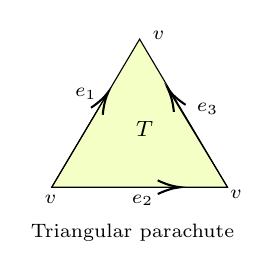
\begin{tikzpicture}[x=0.75pt,y=0.75pt,yscale=-1,xscale=1]
  %uncomment if require: \path (0,300); %set diagram left start at 0, and has height of 300
  
  %Shape: Triangle [id:dp17876379472415316] 
  \draw  [fill={rgb, 255:red, 243; green, 255; blue, 196 }  ,fill opacity=1 ] (267.22,57.33) -- (309.56,128.67) -- (224.89,128.67) -- cycle ;
  %Straight Lines [id:da5263568056898096] 
  \draw    (224.89,128.67) -- (284.89,128.67) ;
  \draw [shift={(286.89,128.67)}, rotate = 180] [color={rgb, 255:red, 0; green, 0; blue, 0 }  ][line width=0.75]    (10.93,-3.29) .. controls (6.95,-1.4) and (3.31,-0.3) .. (0,0) .. controls (3.31,0.3) and (6.95,1.4) .. (10.93,3.29)   ;
  %Straight Lines [id:da6773553420028544] 
  \draw    (309.56,128.67) -- (281.92,83.04) ;
  \draw [shift={(280.89,81.33)}, rotate = 58.8] [color={rgb, 255:red, 0; green, 0; blue, 0 }  ][line width=0.75]    (10.93,-3.29) .. controls (6.95,-1.4) and (3.31,-0.3) .. (0,0) .. controls (3.31,0.3) and (6.95,1.4) .. (10.93,3.29)   ;
  %Straight Lines [id:da2169048756524028] 
  \draw    (224.89,128.67) -- (251.2,84.39) ;
  \draw [shift={(252.22,82.67)}, rotate = 120.72] [color={rgb, 255:red, 0; green, 0; blue, 0 }  ][line width=0.75]    (10.93,-3.29) .. controls (6.95,-1.4) and (3.31,-0.3) .. (0,0) .. controls (3.31,0.3) and (6.95,1.4) .. (10.93,3.29)   ;
  
  % Text Node
  \draw (272.22,52.07) node [anchor=north west][inner sep=0.75pt]  [font=\scriptsize]  {$v$};
  % Text Node
  \draw (220.22,131.4) node [anchor=north west][inner sep=0.75pt]  [font=\scriptsize]  {$v$};
  % Text Node
  \draw (309.56,128.73) node [anchor=north west][inner sep=0.75pt]  [font=\scriptsize]  {$v$};
  % Text Node
  \draw (264.22,95.73) node [anchor=north west][inner sep=0.75pt]  [font=\footnotesize]  {$T$};
  % Text Node
  \draw (262.22,131.07) node [anchor=north west][inner sep=0.75pt]  [font=\scriptsize]  {$e_{2}$};
  % Text Node
  \draw (234.89,79.73) node [anchor=north west][inner sep=0.75pt]  [font=\scriptsize]  {$e_{1}$};
  % Text Node
  \draw (293.56,87.07) node [anchor=north west][inner sep=0.75pt]  [font=\scriptsize]  {$e_{3}$};
  % Text Node
  \draw (213.56,145.33) node [anchor=north west][inner sep=0.75pt]  [font=\scriptsize] [align=left] {Triangular parachute};
  
  
  \end{tikzpicture}
 \end{wrapfigure}
 
\sol \textbf{\textsf{Homology of triangular parachute ($P$)}}:  We will compute the simplicial homology groups of the space $P$. By the equivalence of simplicial and singular homology we will get the singular groups of $P$. It has only one $0$-simplex $v$, three $1$-simplex $e_1,e_2,e_3$ and one $2$ simplex $T$. So the terms of corresponding simplicial chain complex are $\D_0(P) = \Z v$, $\D_1(P) = \Z e_1 \oplus \Z e_2 \oplus \Z e_3$ and $\D_2(T)=\Z T$. We have the following chain complex, $$\cdots 0 \xrightarrow{\p_2} \Z T \xrightarrow{\p_1}\Z e_1 \oplus \Z e_2 \oplus \Z e_3 \xrightarrow{\p_0} \Z v \xrightarrow{} 0$$ It is not hard to see that, $\p_0(e_1) = v-v =\p_0(e_2) = \p_0(e_3)$, so $\operatorname{Im}(\p_0) = 0$ and hence $H_0^{\D}(P) \simeq \Z$. Note that, $\ker \p_0 = \Z e_1 \oplus \Z e_2 \oplus \Z e_3$ and $\operatorname{Im} (\p_1) = \Z \p_1(T) = \Z (e_2+e_3-e_1)$. Thus $$H_1^{\D}(P)= \Z e_1 \oplus \Z e_2 \oplus \Z e_3 / \Z (e_2+e_3-e_1) \simeq \Z \oplus \Z$$ We have $\ker \p_1 = 0$ as there is no way we can get $0$ from $e_2+e_3-e_1$. So, $H_2^{\D}(P) \simeq 0$. So, $$H_n(H) \simeq \begin{cases}
   \Z & \text{ if } n= 0 \\
   \Z^2 &  \text{ otherwise } n=1 \\
   0 & \text{ otherwise }
 \end{cases}$$


  \begin{wrapfigure}{r}{4cm}   
   \centering 


   \tikzset{every picture/.style={line width=0.75pt}} %set default line width to 0.75pt        

   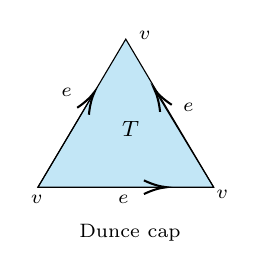
\begin{tikzpicture}[x=0.75pt,y=0.75pt,yscale=-1,xscale=1]
   %uncomment if require: \path (0,300); %set diagram left start at 0, and has height of 300
   
   %Shape: Triangle [id:dp17876379472415316] 
   \draw  [fill={rgb, 255:red, 194; green, 230; blue, 246 }  ,fill opacity=1 ] (267.22,57.33) -- (309.56,128.67) -- (224.89,128.67) -- cycle ;
   %Straight Lines [id:da5263568056898096] 
   \draw    (224.89,128.67) -- (284.89,128.67) ;
   \draw [shift={(286.89,128.67)}, rotate = 180] [color={rgb, 255:red, 0; green, 0; blue, 0 }  ][line width=0.75]    (10.93,-3.29) .. controls (6.95,-1.4) and (3.31,-0.3) .. (0,0) .. controls (3.31,0.3) and (6.95,1.4) .. (10.93,3.29)   ;
   %Straight Lines [id:da6773553420028544] 
   \draw    (309.56,128.67) -- (281.92,83.04) ;
   \draw [shift={(280.89,81.33)}, rotate = 58.8] [color={rgb, 255:red, 0; green, 0; blue, 0 }  ][line width=0.75]    (10.93,-3.29) .. controls (6.95,-1.4) and (3.31,-0.3) .. (0,0) .. controls (3.31,0.3) and (6.95,1.4) .. (10.93,3.29)   ;
   %Straight Lines [id:da2169048756524028] 
   \draw    (224.89,128.67) -- (251.2,84.39) ;
   \draw [shift={(252.22,82.67)}, rotate = 120.72] [color={rgb, 255:red, 0; green, 0; blue, 0 }  ][line width=0.75]    (10.93,-3.29) .. controls (6.95,-1.4) and (3.31,-0.3) .. (0,0) .. controls (3.31,0.3) and (6.95,1.4) .. (10.93,3.29)   ;
   
   % Text Node
   \draw (272.22,52.07) node [anchor=north west][inner sep=0.75pt]  [font=\scriptsize]  {$v$};
   % Text Node
   \draw (220.22,131.4) node [anchor=north west][inner sep=0.75pt]  [font=\scriptsize]  {$v$};
   % Text Node
   \draw (309.56,128.73) node [anchor=north west][inner sep=0.75pt]  [font=\scriptsize]  {$v$};
   % Text Node
   \draw (264.22,95.73) node [anchor=north west][inner sep=0.75pt]  [font=\footnotesize]  {$T$};
   % Text Node
   \draw (262.22,131.07) node [anchor=north west][inner sep=0.75pt]  [font=\scriptsize]  {$e$};
   % Text Node
   \draw (234.89,79.73) node [anchor=north west][inner sep=0.75pt]  [font=\scriptsize]  {$e$};
   % Text Node
   \draw (293.56,87.07) node [anchor=north west][inner sep=0.75pt]  [font=\scriptsize]  {$e$};
   % Text Node
   \draw (243.56,145.33) node [anchor=north west][inner sep=0.75pt]  [font=\scriptsize] [align=left] {Dunce cap};
   
   
   \end{tikzpicture}        
   
 
  \end{wrapfigure}

  \vspace*{0.2cm}

\noindent \textbf{\textsf{Homology groups of Dunce cap ($H$)}}:
 We will compute the simplicial homology groups of the space $H$. By the equivalence of simplicial and singular homology we will get the singular groups of $H$. The $0$-simplex of $H$ is only $v$ as it has only one vertex. $1$-simplex of $H$ is the edges $e$ (as all the edges in $D^2$ are identified to get $H$). It has only one $2$-simplex $T$ that comes from $D^2$ and it has no other higher simplicial structure. So the terms of simplicial chain complexes are, $\D_0(H) = \Z v$, $\D_1(H) = \Z e$ and $\D_2(H)= \Z T$ and $\D_n(H) \simeq 0$, for $n \geq 3$. We have the following chain complex, $$0 \xrightarrow{\p_2} \Z T \xrightarrow{\p_1}\Z e \xrightarrow{\p_0} \Z v \xrightarrow{} 0$$ We have $\operatorname{Im} (\p_0)= \p_0 (e) = v-v =0$ so, $H_0^{\D} (H) \simeq \Z$. So we have $\ker \p_0 = \Z e$ and $\operatorname{Im}(\p_1) = \Z \p_1(T) = \Z e$. Thus $H_1^{\D}(H) = 0$. From the last part we can say $\ker \p_1 = 0$ and hence $H_2^{\D} (H)=0$. So, $$H_n(H) \simeq \begin{cases}
   \Z & \text{ if } n= 0 \\
   0 &  \text{ otherwise }
 \end{cases}$$

\vspace*{0.2cm}

\noindent From the above two computations we can see $1$-st homology group of the spaces $H$ and $P$ are different. so, $H$ and $P$ can't be homotopy equivalent. $\hfill \blacksquare$


\end{document} 

